\documentclass[tikz,border=6pt]{standalone}
\usepackage{amsmath,amssymb}
\usetikzlibrary{shapes.geometric,arrows.meta,positioning,fit,backgrounds,calc}

% --- small red/orange flame icon used to mark trainable modules ---
\newcommand{\flame}[1]{%
  \begin{scope}[shift={#1},scale=0.22,line width=0.5pt]
    \draw[fill=red!75!orange,draw=red!45!black]
      (0,0) .. controls (-2.7,2.6) and (-2.1,6.6) .. (0,9.6)
            .. controls (2.4,6.4) and (2.7,2.4) .. (0,0) -- cycle;
    \draw[fill=yellow!80!orange,draw=none]
      (0,0.9) .. controls (-1.15,2.6) and (-0.95,4.9) .. (0,7.1)
            .. controls (1.1,4.7) and (1.15,2.5) .. (0,0.9) -- cycle;
  \end{scope}
}
% --- trainable-module badge: small circle sitting exactly on the box border, like the frozen (*) badge ---
\newcommand{\trainbadge}[1]{%
  \node[circle,draw=red!55!black,fill=white,minimum size=3.6mm,inner sep=0pt,line width=0.4pt] at #1 {};
  \flame{($#1+(0,-1.05)$)}
}

\begin{document}
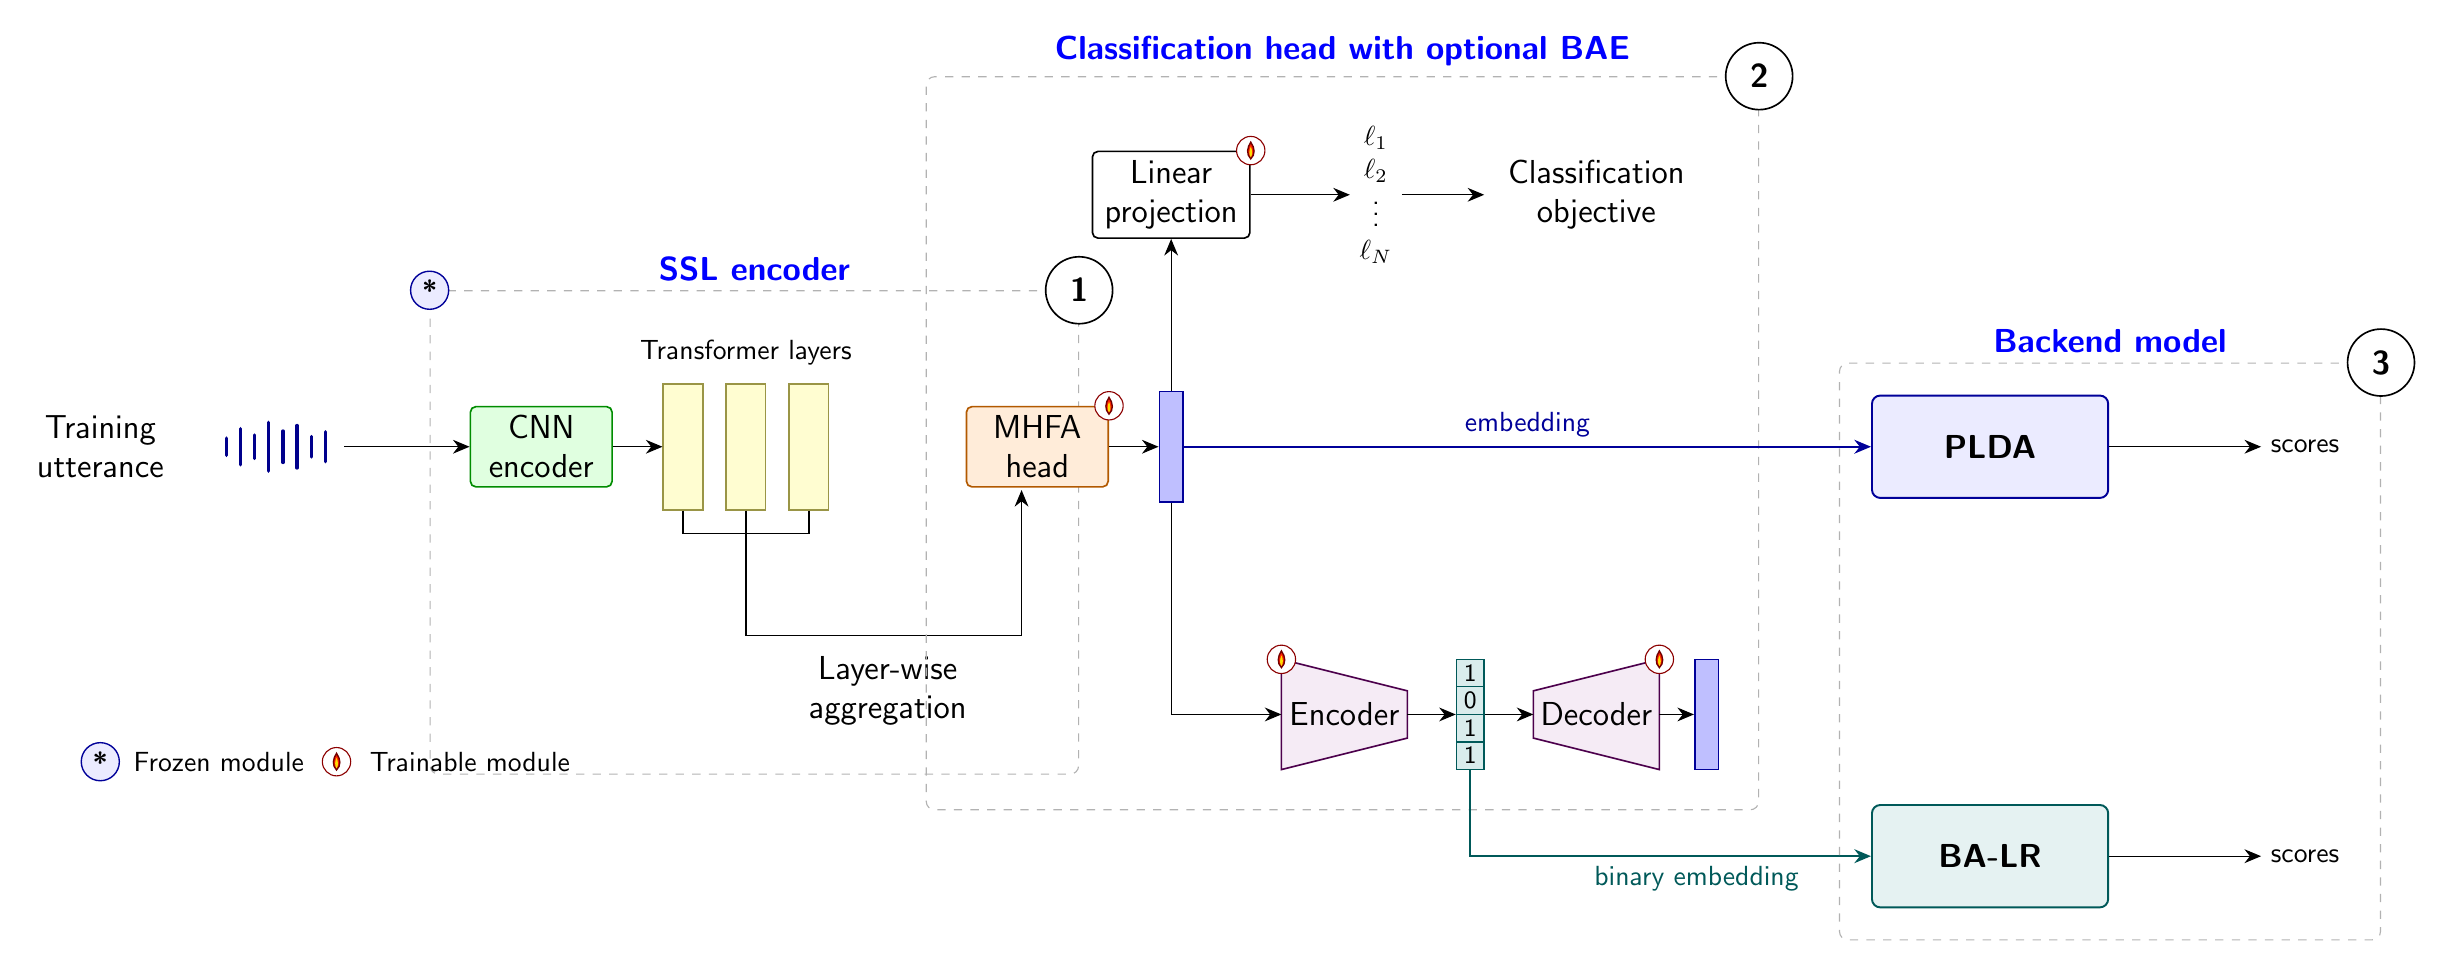
\begin{tikzpicture}[
  x=1mm,y=1mm,
  font=\sffamily\large,
  >={Stealth[length=6pt,width=5pt]},
  every node/.style={align=center},
  cnnbox/.style={rectangle,rounded corners=2pt,draw=green!55!black,fill=green!12,
    minimum width=18mm,minimum height=9mm,line width=0.6pt},
  transbox/.style={rectangle,draw=yellow!55!black,fill=yellow!18,
    minimum width=5mm,minimum height=16mm,line width=0.6pt},
  mhfabox/.style={rectangle,rounded corners=2pt,draw=orange!70!black,fill=orange!15,
    minimum width=18mm,minimum height=10mm,line width=0.6pt},
  linbox/.style={rectangle,rounded corners=2pt,draw=black,fill=white,
    minimum width=20mm,minimum height=9mm,line width=0.6pt},
  embvec/.style={rectangle,draw=blue!60!black,fill=blue!25,minimum width=3mm,minimum height=14mm,line width=0.6pt},
  backendbox/.style={rectangle,rounded corners=3pt,draw=black,line width=0.7pt,
    minimum width=30mm,minimum height=13mm,font=\sffamily\bfseries\large},
  modtitle/.style={font=\sffamily\bfseries\large,text=blue},
  frozenmark/.style={circle,draw=blue!60!black,fill=blue!8,inner sep=1.6pt,line width=0.5pt,font=\sffamily\normalsize},
  badge/.style={circle,draw=black,fill=white,minimum size=8.5mm,inner sep=0pt,font=\sffamily\bfseries\large,line width=0.6pt},
]

%======================================================================
% MODULE 1 -- SPEECH ENCODER
%======================================================================
\node (wave) at (-40,0) {Training\\utterance};

% --- realistic waveform icon ---
\foreach \i/\h in {0/2.2,1/4.6,2/3.0,3/6.2,4/4.0,5/5.4,6/2.6,7/3.8}{
  \draw[very thick,cap=round,blue!55!black] (-24+\i*1.8,-\h/2) -- (-24+\i*1.8,\h/2);
}

\node[cnnbox] (cnn) at (16,0) {CNN\\encoder};
\draw[->] (-9,0) -- (cnn.west);

\node[transbox] (t1) at (34,0) {};
\node[transbox] (t2) at (42,0) {};
\node[transbox] (t3) at (50,0) {};
\node[font=\sffamily\normalsize] (tlabel) at (42,12) {Transformer layers};

\draw[->] (cnn.east) -- (t1.west);

\node[font=\sffamily\large,text width=36mm] (aggnote) at (60,-31) {Layer-wise aggregation};
\foreach \n in {t1,t2,t3}{\draw (\n.south) -- ++(0,-3);}
\draw (34,-11) -- (50,-11);
\draw (42,-11) -- (42,-24);
\draw[->] (42,-24) -- (77,-24) -- (77,-5.5);
\coordinate (aggline) at (42,-24);

\node[fit=(cnn)(t1)(t2)(t3)(tlabel)(aggnote)(aggline), draw=gray!60, dashed, rounded corners=3pt,
      inner sep=5mm] (sslbox) {};
\node[modtitle] at (sslbox.north) [above] {SSL encoder};
\node[frozenmark] at (sslbox.north west) {\bfseries *};
\node[badge] at (sslbox.north east) {1};

%======================================================================
% MODULE 2 -- CLASSIFICATION HEAD (+ optional BAE)
%======================================================================
\node[mhfabox] (mhfa) at (79,0) {MHFA\\head};
\trainbadge{(mhfa.north east)}

\node[embvec] (emb) at (96,0) {};
\draw[->] (mhfa.east) -- (emb.west);

% --- branch up: linear projection + language-classification objective ---
\node[linbox] (lin) at (96,32) {Linear\\projection};
\draw[->] (emb.north) -- (lin.south);
\trainbadge{(lin.north east)}

\node[font=\sffamily\normalsize] (logits) at (122,32) {$\ell_1$\\$\ell_2$\\$\vdots$\\$\ell_N$};
\draw[->] (lin.east) -- (logits.west);
\node[font=\sffamily\large,text width=26mm] (clsobj) at (150,32) {Classification objective};
\draw[->] (logits.east) -- (clsobj.west);

% --- branch down: optional Binary AutoEncoder (symmetric encoder/decoder) ---
\coordinate (encL) at (110,-34);   % tall (input) edge of the encoder
\coordinate (encLt) at (110,-27);
\coordinate (encLb) at (110,-41);
\coordinate (encR)  at (126,-34); % narrow (output) edge of the encoder
\coordinate (encRt) at (126,-31);
\coordinate (encRb) at (126,-37);
\draw[fill=violet!8,draw=violet!60!black,line width=0.6pt]
  (encLt) -- (encLb) -- (encRb) -- (encRt) -- cycle;
\node[font=\sffamily\large] at (118,-34) {Encoder};
\draw[->] (emb.south) |- (encL);
\trainbadge{(encLt)}

\node[rectangle,draw=teal!70!black,fill=teal!15,line width=0.6pt,
      minimum width=3.5mm,minimum height=14mm] (code) at (134,-34) {};
\foreach \yy in {-30.5,-34,-37.5}{\draw[teal!70!black,line width=0.4pt] (132.25,\yy) -- (135.75,\yy);}
\node[font=\sffamily\small] at (134,-28.75) {1};
\node[font=\sffamily\small] at (134,-32.25) {0};
\node[font=\sffamily\small] at (134,-35.75) {1};
\node[font=\sffamily\small] at (134,-39.25) {1};
\draw[->] (encR) -- (code.west);

\coordinate (decL)  at (142,-34); % narrow (input) edge of the decoder -- mirrors the encoder
\coordinate (decLt) at (142,-31);
\coordinate (decLb) at (142,-37);
\coordinate (decR)  at (158,-34); % tall (output) edge of the decoder
\coordinate (decRt) at (158,-27);
\coordinate (decRb) at (158,-41);
\draw[fill=violet!8,draw=violet!60!black,line width=0.6pt]
  (decLt) -- (decLb) -- (decRb) -- (decRt) -- cycle;
\node[font=\sffamily\large] at (150,-34) {Decoder};
\draw[->] (code.east) -- (decL);
\trainbadge{(decRt)}

\node[embvec] (rec) at (164,-34) {};
\draw[->] (decR) -- (rec.west);

\node[fit=(mhfa)(lin)(clsobj)(logits)(encLt)(encLb)(decRt)(decRb)(code)(rec)(emb), draw=gray!60, dashed,
      rounded corners=3pt, inner sep=5mm] (headbox) {};
\node[modtitle] at (headbox.north) [above] {Classification head with optional BAE};
\node[badge] at (headbox.north east) {2};

%======================================================================
% MODULE 3 -- BACKEND
%======================================================================
\node[backendbox,fill=blue!8,draw=blue!60!black] (plda) at (200,0) {PLDA};
\node[backendbox,fill=teal!10,draw=teal!70!black] (balr) at (200,-52) {BA-LR};

\draw[->,blue!60!black,thick] (emb.east) -- (plda.west)
      node[midway,above,font=\sffamily\normalsize,align=center] {embedding};
\draw[->,teal!70!black,thick] (code.south) -- (134,-52) -- (balr.west)
      node[near start,below,font=\sffamily\normalsize,align=center,xshift=16mm] {binary embedding};

\node[font=\sffamily\normalsize,align=left] (out1) at (240,0) {scores};
\node[font=\sffamily\normalsize,align=left] (out2) at (240,-52) {scores};
\draw[->] (plda.east) -- (out1.west);
\draw[->] (balr.east) -- (out2.west);

\node[fit=(plda)(balr)(out1)(out2), draw=gray!60, dashed, rounded corners=3pt,
      inner sep=4mm] (backbox) {};
\node[modtitle] at (backbox.north) [above] {Backend model};
\node[badge] at (backbox.north east) {3};

%======================================================================
% LEGEND
%======================================================================
\node[frozenmark] (lfrozen) at (-40,-40) {\bfseries *};
\node[font=\sffamily\normalsize,anchor=west] at (-37,-40) {Frozen module};
\trainbadge{(-10,-40)}
\node[font=\sffamily\normalsize,anchor=west] at (-7,-40) {Trainable module};

\end{tikzpicture}
\end{document}
